% ----------------------------------------------------------------
% AMS-LaTeX Paper ************************************************
% **** -----------------------------------------------------------
\documentclass[10pt]{amsart}
%\textwidth 14.5cm
%\textheight 22cm
%\hoffset -1.5cm
%\voffset -2.2cm
\usepackage{graphicx}
\usepackage{latexsym}
\usepackage{amsfonts}
\usepackage{amsthm}
\usepackage{amssymb}
\usepackage{amsmath}
\usepackage{enumerate}
\usepackage{color}
\usepackage{stmaryrd}
\usepackage{chemarrow}
\usepackage[all]{xy}
\usepackage[pdftex,bookmarksnumbered,bookmarksopen,colorlinks,linkcolor=blue,anchorcolor=black,citecolor=blue,urlcolor=blue]{hyperref}
\usepackage{booktabs}
\usepackage{makecell}
\usepackage{subfigure}

%\usepackage{mathabx}
% ----------------------------------------------------------------
\vfuzz2pt % Don't report over-full v-boxes if over-edge is small
\hfuzz2pt % Don't report over-full h-boxes if over-edge is small
% THEOREMS -------------------------------------------------------
\newtheorem{thm}{Theorem}[section]
\newtheorem{cor}[thm]{Corollary}
\newtheorem{lem}[thm]{Lemma}
\newtheorem{prop}[thm]{Proposition}
\theoremstyle{definition}
\newtheorem{defn}[thm]{Definition}
\theoremstyle{remark}
\newtheorem{rem}[thm]{Remark}
%\numberwithin{equation}{section}
% MATH -----------------------------------------------------------
\newcommand{\norm}[1]{\left\Vert#1\right\Vert}
\newcommand{\abs}[1]{\left\vert#1\right\vert}
\newcommand{\set}[1]{\left\{#1\right\}}
\newcommand{\Real}{\mathbb R}
\newcommand{\eps}{\varepsilon}
\newcommand{\To}{\longrightarrow}
\newcommand{\BX}{\mathbf{B}(X)}
\newcommand{\A}{\mathcal{A}}

\newcommand{\dx}{\,{\rm d}x}
\newcommand{\dd}{\,{\rm d}}
\newcommand{\bs}{\boldsymbol}
\newcommand{\mcal}{\mathcal}

\DeclareMathOperator*{\img}{img}
%\DeclareMathOperator*{\span}{span}
\newcommand{\sign}{\operatorname{sign}}
\newcommand{\curl}{\operatorname{curl}}
\renewcommand{\div}{\operatorname{div}}
%\renewcommand{\grad}{\operatorname{grad}}
\newcommand{\grad}{\operatorname{grad}}
\newcommand{\tr}{\operatorname{tr}}
% \DeclareMathOperator*{\tr}{tr}
\DeclareMathOperator*{\rot}{rot}
\DeclareMathOperator*{\var}{Var}
\newcommand{\dev}{\operatorname{dev}}
\newcommand{\sym}{\operatorname{sym}}
\newcommand{\skw}{\operatorname{skw}}
\newcommand{\spn}{\operatorname{spn}}
\newcommand{\mspn}{\operatorname{mspn}}
\newcommand{\mskw}{\operatorname{mskw}}
\newcommand{\vskw}{\operatorname{vskw}}
\newcommand{\vspn}{\operatorname{vspn}}
\newcommand{\defm}{\operatorname{def}}
\newcommand{\hess}{\operatorname{hess}}
% ----------------------------------------------------------------
\begin{document}

\title{\large Detailed Response to Referees}%

\date{}%
%\dedicatory{}%
%\commby{}%
% ----------------------------------------------------------------

\maketitle

\begin{enumerate}[1.]

\item \textsf{
in the numerical section; I agree that it is important to check the rate of
convergence of the method;}

\textsf{However, the convergence does not automatically
guarantee the invertibility of the local stiffness matrices, as imposing the
Dirichlet boundary conditions may have a “stabilizing effect”. So, you should
investigate the number of zero eigenvalues of the local stiffness matrix.}

\textsf{For instance, pick three different hexagonal elements with a fixed degree of
accuracy, e.g., k = 3: the first being a regular hexagon; the second being a
quasi-regular hexagon (small perturbation of the previous element); the third
being a square with an edge containing two hanging nodes. Check whether the
stiffness matrix always has only one zero eigenvalue, i.e., the method is indeed
stabilization free; 
}

\smallskip \noindent \textcolor[rgb]{1.00,0.00,0.00}{Reply.}
\begin{figure}[h]
\centering
\subfigure{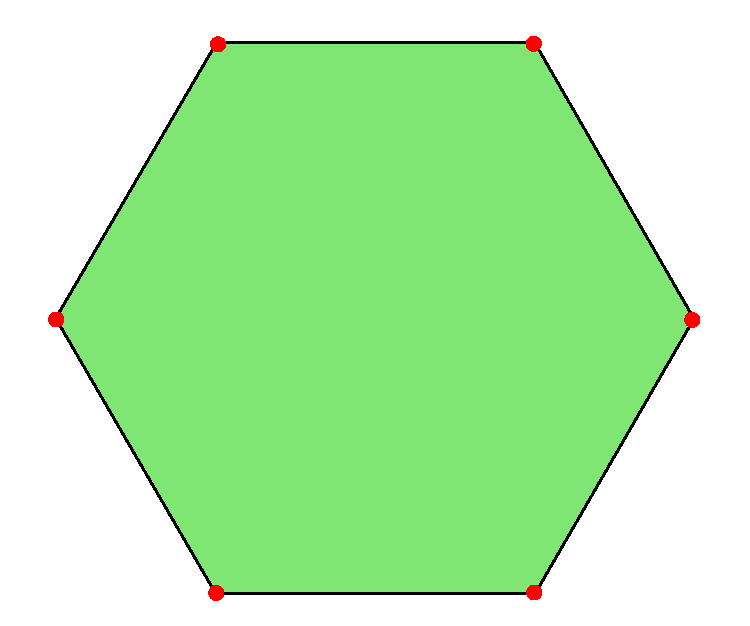
\includegraphics[width=1.6in]{../figures/hexagon0.pdf}}
    % \caption{Type I:5 tetrahedra}
%%
\subfigure{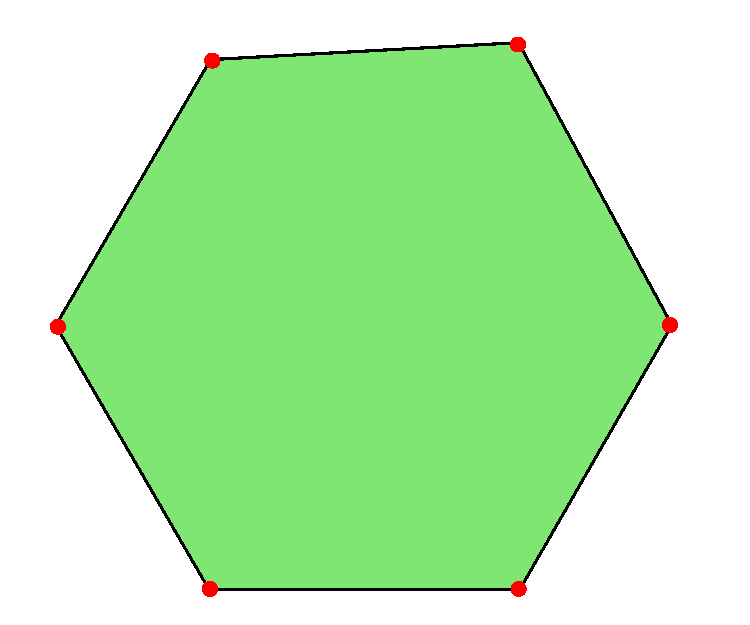
\includegraphics[width=1.6in]{../figures/hexagon1.pdf}}
     %\caption{Type II: 24 tetrahedra}
%%
\subfigure{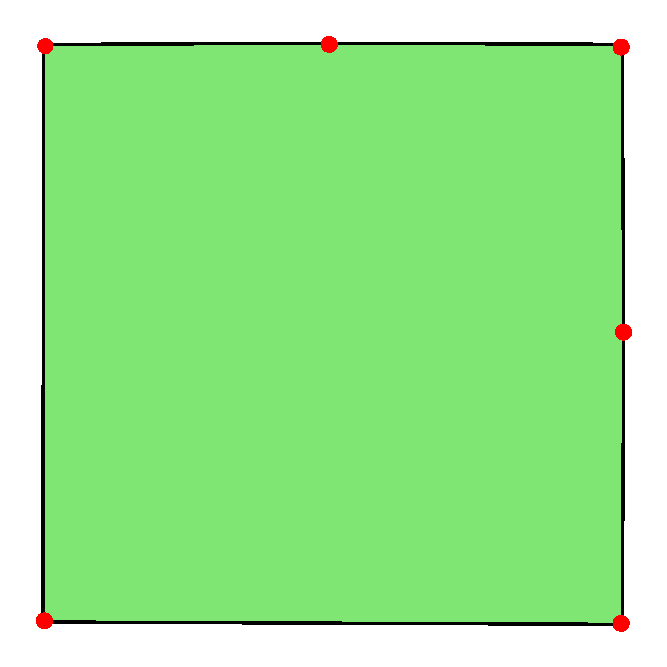
\includegraphics[width=1.3in]{../figures/hexagon2.pdf}}
     %\caption{Trirectangular tetrahedron}
%%
\caption{The regular hexagon(Left), the quasi-regular hexagon generated by regular
    hexagon with a small perturbation (Middle), 
and the square with two hanging nodes (Right)}
  \label{fig:hexagon} %% label for entire figure
\end{figure}

We followed the reviewer's suggestion and constructed three different hexagonal
elements, shown in Figure \ref{fig:hexagon}, and calculated the eigenvalues of local stiffness
matrices. Our numerical results show that, on each element, the number of zero
eigenvalues is only one, indicating that the method is stabilization-free. The
minimum non-zero eigenvalue and the maximum eigenvalue for each element are
shown in Table \ref{tab:comparison0}-\ref{tab:comparison2}:

\begin{table}[h]
\centering
\caption{Comparison of Eigenvalues and Condition Numbers on regular hexagon.}
\label{tab:comparison0}
\begin{tabular}{|l|c|c|c|}
\hline
\textbf{Method} & \textbf{Maximum Eigenvalue} & \textbf{Smallest Nonzero
Eigenvalue} & \textbf{Condition Number} \\ \hline
\thead{Standard \\ nonconforming} & 975.5693189 & 0.309674737 & 3150.303211 \\ \hline
\thead{Standard \\ conforming} & 1012.488116 & 0.297206358 & 3406.683909 \\ \hline
\thead{Stabilization-Free \\ nonconforming} & 992.5956147 & 0.318932029 & 3112.248147 \\ \hline
\thead{Stabilization-Free \\ conforming} & 1011.173331 & 0.298509692 & 3387.405362 \\ \hline
\end{tabular}
\end{table}

\begin{table}[h]
\centering
\caption{Comparison of Eigenvalues and Condition Numbers of quasi-regular hexagon}
\label{tab:comparison1}
\begin{tabular}{|l|c|c|c|}
\hline
\textbf{Method} & \textbf{Maximum Eigenvalue} & \textbf{Smallest Nonzero
Eigenvalue} & \textbf{Condition Number} \\ \hline
\thead{Standard \\ nonconforming} & 935.2883848 & 0.279027715 & 3351.955143 \\ \hline
\thead{Standard \\ conforming} & 1014.672395 & 0.257370621 & 3942.456177 \\ \hline
\thead{Stabilization-Free \\ nonconforming} & 997.4831245 & 0.282126359 & 3535.589964 \\ \hline
\thead{Stabilization-Free \\ conforming} & 1047.876056 & 0.258970708 & 4046.311124 \\ \hline
\end{tabular}
\end{table}

\begin{table}[h]
\centering
\caption{Comparison of Eigenvalues and Condition Numbers of quasi-regular hexagon}
\label{tab:comparison2}
\begin{tabular}{|l|c|c|c|}
\hline
\textbf{Method} & \textbf{Maximum Eigenvalue} & \textbf{Smallest Nonzero
Eigenvalue} & \textbf{Condition Number} \\ \hline
\thead{Standard \\ nonconforming} & 946.6384135 & 0.314530883 & 3009.683513 \\ \hline
\thead{Standard \\conforming} & 983.6588841 & 0.301873276 & 3258.51595 \\ \hline
\thead{Stabilization-Free \\nonconforming} & 963.7580188 & 0.32421634 & 2972.576947 \\ \hline
\thead{Stabilization-Free\\ conforming} & 982.0847615 & 0.303273885 & 3238.276718 \\ \hline
\end{tabular}
\end{table}


\item \textsf{
my feeling is that the proposed stabilization-free approach is much more
expensive than the standard one. Thus, you should check the assembling time
of the stabilization-free and standard VEMs, on: (i) a (reasonably large)
sequence of meshes; (ii) fixing a mesh, increasing the degree of accuracy,
e.g., up to $k = 10$.
}

\smallskip \noindent \textcolor[rgb]{1.00,0.00,0.00}{Reply.}
We have performed the tests on a reasonably large sequence of meshes and fixed a
mesh while increasing the degree of accuracy up to $p = 9$, all experiments were
conducted on a PC with AMD Ryzen 5 3500U CPU and 64-bit Ubuntu 22.04 
operating system. 

The results shown in Table \ref{tab:ptime}, \ref{tab:ttime}, that
for non-conforming elements, stabilization-free method and the standard method 
have similar assembling times. However, for conforming elements,
stabilization-free method
requires additional time due to the projection to a higher degree of polynomial
space.

\begin{table}
\label{tab:ptime}
\caption{Comparison of four methods in assembling stiffness matrix time with
element size $h=0.1$, $p = \{2, 3, 4, 5, 6, 7, 8, 9\}$.}
\centering
\begin{tabular}{|c|c|c|c|c|}
\hline
$p$ & 2 & 3 & 4 & 5 \\ \hline
  \thead{Standard\\nonconforming}& 0.035768747 & 0.067565441 &
 0.134479761 & 0.266502142 \\ \hline
 \thead{Standard\\conforming} & 0.035797358 & 0.068657637 &
 0.13819623 & 0.265289545 \\ \hline
 \thead{Stabilization-Free \\ nonconforming} & 0.060856819 & 0.074303389 & 0.144818068 & 
 0.255729675 \\ \hline 
 \thead{Stabilization-Free \\ conforming} & 0.086450338 & 0.168139219 & 0.294021606 &
 0.544180155 \\ \hline 
$p$ & 6 & 7 & 8 & 9 \\ \hline
  \thead{Standard\\nonconforming} & 1.013250589 & 1.882751942 & 3.374693632 &
  5.522083759 \\ \hline
 \thead{Standard\\conforming} & 0.47455287 & 0.876257181 & 1.737621069 &
 3.04714179 \\ \hline
 \thead{Stabilization-Free \\ nonconforming} & 0.543116093 & 1.009181261 &
 1.954544544 & 3.539043427 \\ \hline
 \thead{Stabilization-Free \\ conforming} & 0.568083763 & 1.030921936 &
 1.984176874 & 3.548179626 \\ \hline
\end{tabular}
\end{table}

\begin{table}
\label{tab:ttime}
\caption{Comparison of four methods in assembling stiffness matrix time with
element size $h=\{1, 0.5, 0.25, 0.125, 0.0625, 0.03125\}$, $p = 5$.}
\begin{tabular}{|c|c|c|c|c|c|c|}
\hline
h & 1 & 0.5 & 0.25 & 0.125 & 0.0625 & 0.03125 \\
\hline
  \thead{Standard\\nonconforming} & 0.01217103 & 0.022562504 & 0.056048393 & 0.171028852 & 0.569516897 & 2.440380812 \\
\hline
  \thead{Standard\\nonconforming} & 0.012936115 & 0.023290396 & 0.057774305 & 0.178972006 & 0.587247849 & 2.411020279 \\
\hline
\thead{Stabilization-Free \\ nonconforming}& 0.011769056 & 0.024716616 & 0.065015793 & 0.182201147 & 0.588429689 & 2.283073902 \\
\hline
\thead{Stabilization-Free \\ conforming} & 0.023740768 & 0.052335024 & 0.144128084 & 0.377803564 & 1.287475586 & 5.004751682 \\
\hline
\end{tabular}
\end{table}

\begin{figure}[h]
\centering
\subfigure{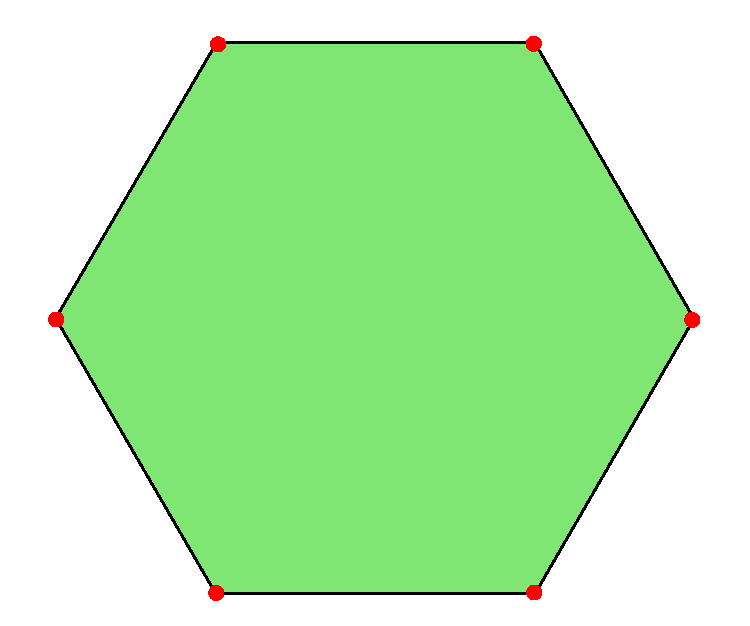
\includegraphics[width=1.6in]{../figures/hexagon0.pdf}}
    % \caption{Type I:5 tetrahedra}
%%
\subfigure{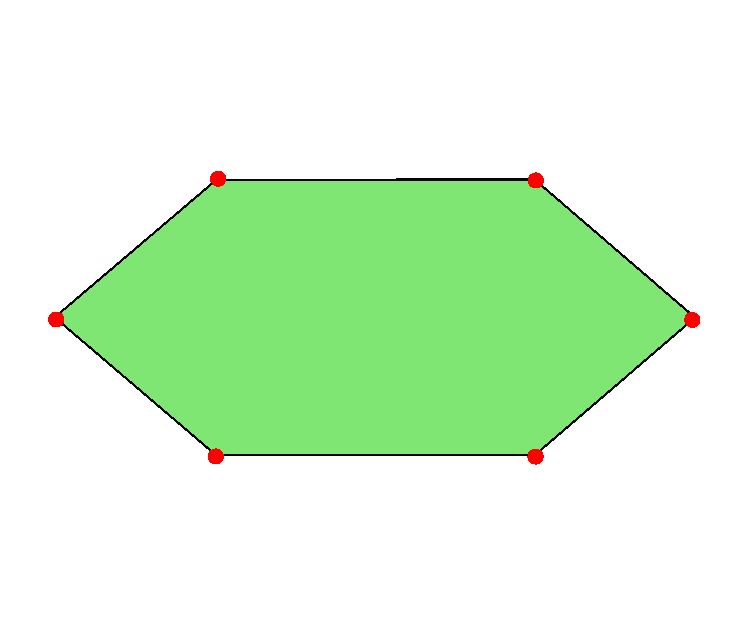
\includegraphics[width=1.6in]{../figures/hexagon3.pdf}}
     %\caption{Type II: 24 tetrahedra}
%%
\subfigure{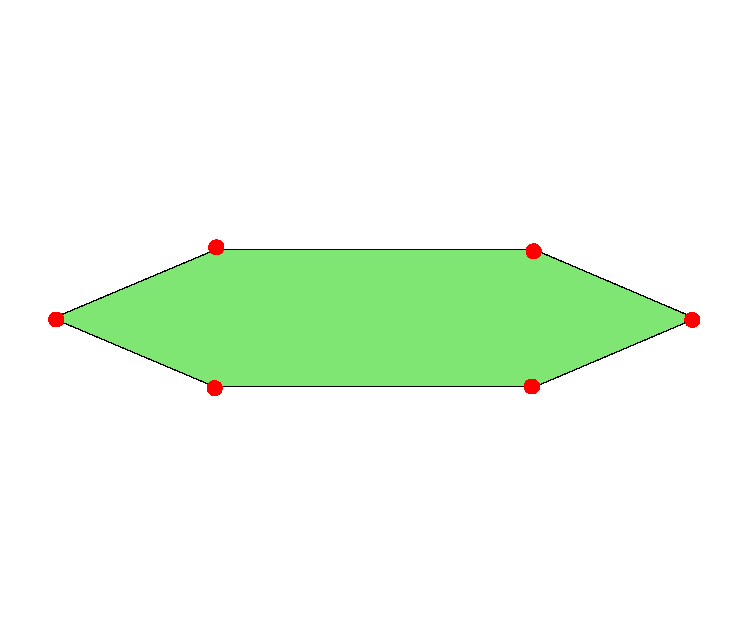
\includegraphics[width=1.3in]{../figures/hexagon4.pdf}}
     %\caption{Trirectangular tetrahedron}
%%
\caption{The hexagon $H_0, H_1, H_2$}
  \label{fig:collapsehexagon} %% label for entire figure
\end{figure}

\item \textsf{
along the same avenue, you should also compare the condition number of the
global matrices obtained with the two approaches in the two situations (i) and
(ii) above. Furthermore, you may also wish to consider sequences of meshes with
“collapsing elements” (refine a mesh and change the aspect ratio), and check the
condition numbers again.  As a suggestion, since the condition number should be
computed scaling the diagonal of the matrix, you can empirically check such
conditioning by testing the two approaches on a patch test. The conditioning can
be estimated checking the growth of the error for the patch test.
}

\smallskip \noindent \textcolor[rgb]{1.00,0.00,0.00}{Reply.}
We designed two experiments to estimate the condition number of the stiffness
matrix. Firstly, we consider a hexagonal sequence $\{H_i\}_{i=0}^{\infty}$, the
vertices of $H_i$ as follow :

$$
A_i = (1, 0), B_i = (0.5, a_i), C_i = (-0.5, a), D_i=(-1, 0), 
$$
$$
E_i = (-0.5, -a_i), F_i = (0.5, -a_i)
$$

where $a_i = \frac{\sqrt{3}}{2^{i+1}}$, the image of $\{H_0, H_1, H_2\}$ shown
in Figure 3. 
We construct virtual element space on $K_i$, the condition number of stiffness
matrix derive by different methods shown in Figure
\ref{fig:collapsehexagon_conditionnumber}, where the four lines
almost coincide, the condition numbers obtained from both methods are same.

\begin{figure}[h]
\centering
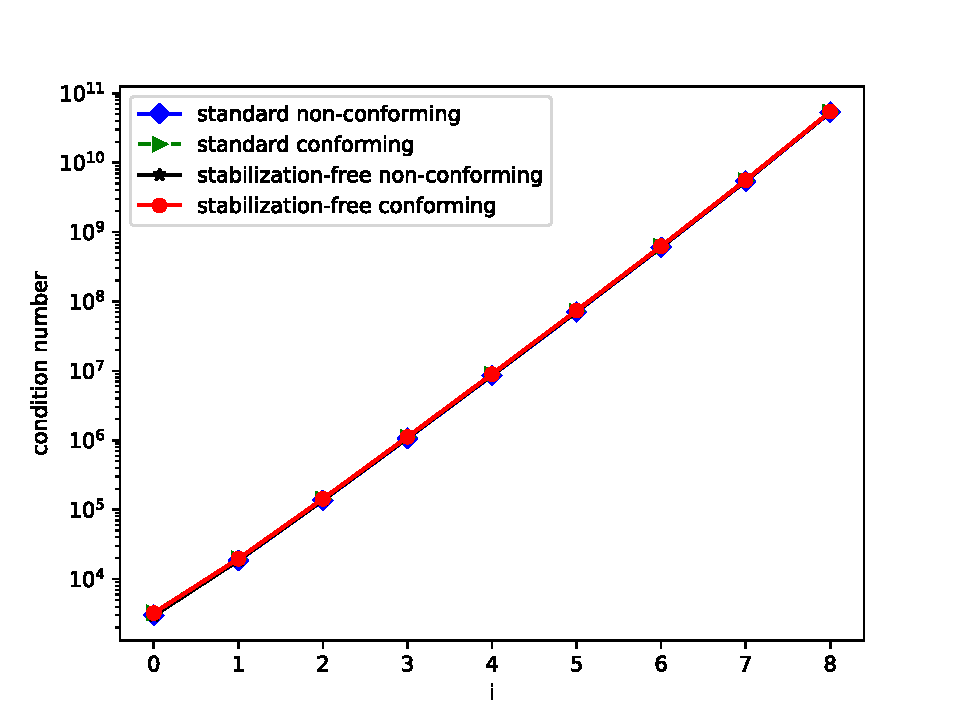
\includegraphics[width=3.0in]{../figures/collapsing_condition_number.pdf}
\caption{The condition number of four method on collapsing hexagon.}
  \label{fig:collapsehexagon_conditionnumber} %% label for entire figure
\end{figure}

Secondly,  consider the patch test problems:

$$
\left\{\begin{aligned}
-\Delta u & = 0 \quad x \in \Omega\\
u & = g \quad x \in \partial \Omega
\end{aligned}\right.
$$

where $\Omega = (0, 1)^2, \ u = g = 1+x+y$. 

Set $h_x$ is size of mesh in the x-direction, $h_y$ is size of mesh in the
y-direction, p is degree of accuracy, 
we observe the behavior of $L^2$ errors $||u - u_h||_0$ of patch test in the following three ways:
\begin{enumerate}[(1)]
\item Fix $h_x=h_y=0.2$, change $p= 1, 2, 3, 4, 5, 6, 7, 8, 9$.
\item Fix $p=3$, change $h_x=h_y=\frac{1}{2}, \frac{1}{4}, \frac{1}{8},
    \frac{1}{16}, \frac{1}{32}$.
\item Fix $p=3$, $h_x=0.2$, change $h_y=\frac{1}{2}, \frac{1}{4}, \frac{1}{8},
    \frac{1}{16}, \frac{1}{32}, \frac{1}{64}, \frac{1}{128}, \frac{1}{256}$.
\end{enumerate}

The errors are shown in Figure \ref{fig:patchtest}, where 
the errors of standard method and stabilization-free method are similar. 
Furthermore, 
the condition numbers of the stiffness matrix obtained by
standard method and stabilization-free method are similar, because of the error
of the patch test is affected by the condition number.


\begin{figure}[h]
\centering
\subfigure{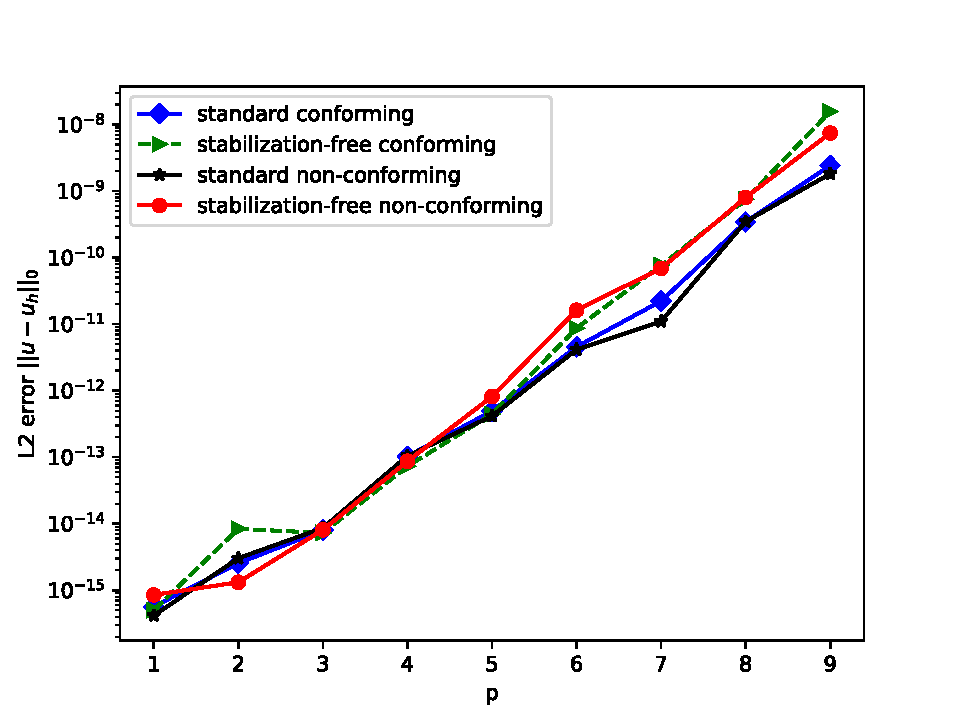
\includegraphics[width=1.6in]{../figures/patch_test_p.pdf}}
    % \caption{Type I:5 tetrahedra}
%%
\subfigure{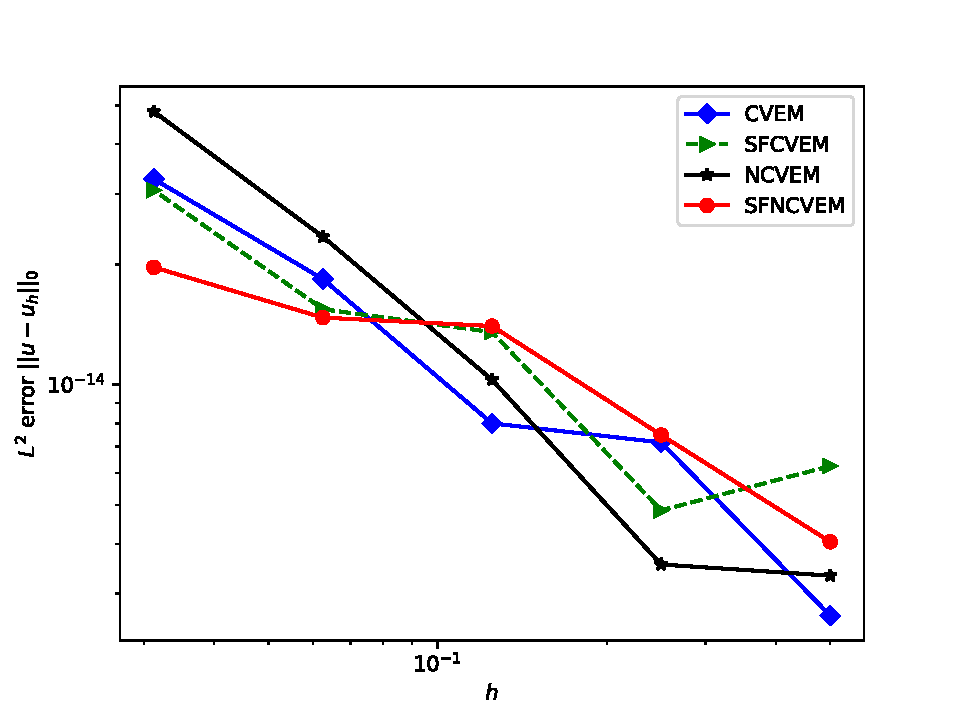
\includegraphics[width=1.6in]{../figures/patch_test_h.pdf}}
     %\caption{Type II: 24 tetrahedra}
%%
\subfigure{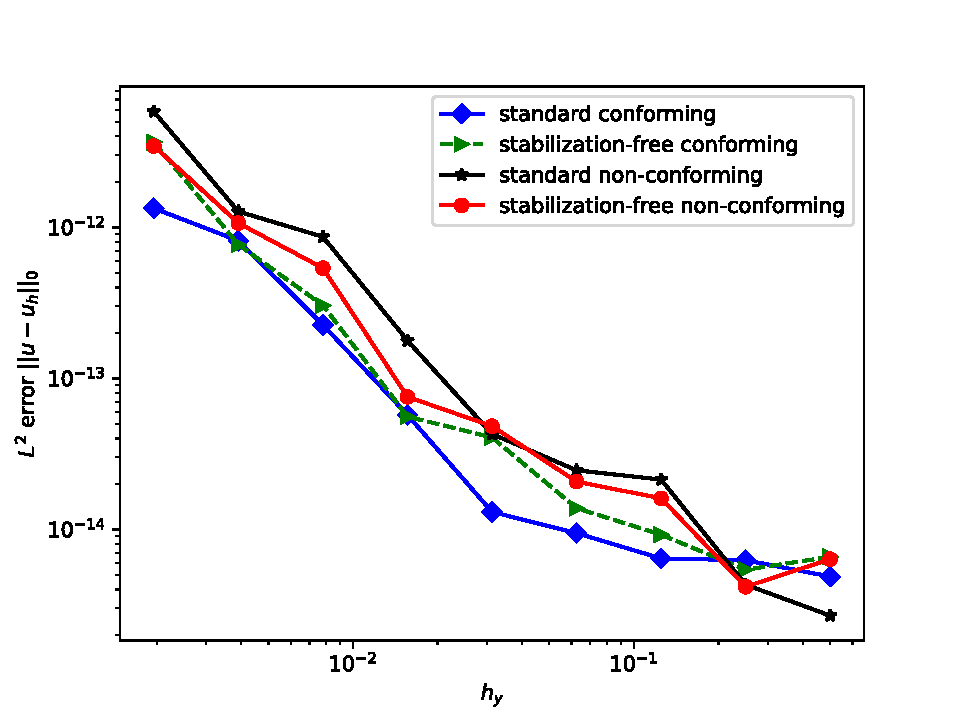
\includegraphics[width=1.6in]{../figures/patch_test_hy.pdf}}
     %\caption{Trirectangular tetrahedron}
%%
\caption{The $L^2$ error of patch test.}
  \label{fig:patchtest} %% label for entire figure
\end{figure}


















\end{enumerate}

\end{document}
